\documentclass[11pt,a4paper]{article}

\usepackage{graphicx}
\usepackage[table]{xcolor}
\usepackage[left=2.3cm, right=2.3cm, top=2.4cm, bottom=2.4cm]{geometry}
\usepackage{amsmath,amssymb,amsthm}
\usepackage{fontspec}
\setmainfont{Liberation Serif}
\setsansfont{Liberation Sans}
\setmonofont{Liberation Mono}[Scale=0.86]
\usepackage[russian]{babel}
\usepackage{booktabs}
\usepackage{tabularx}
\newcolumntype{Y}{>{\raggedright\arraybackslash}X}
\usepackage{colortbl}
\usepackage{enumitem}
\usepackage{tcolorbox}
\definecolor{linkblue}{HTML}{1e3a5f}
\definecolor{accgreen}{HTML}{0e7c66}
\definecolor{warnamber}{HTML}{b45309}
\definecolor{rowlight}{HTML}{f0f5fa}
\usepackage[colorlinks=true, linkcolor=linkblue, urlcolor=linkblue, unicode=true]{hyperref}
\setlist{nosep}
\tolerance=1200
\emergencystretch=2.5em

\newcommand{\dd}{\mathrm{d}}
\newcommand{\kap}{\kappa_{\mathrm{cyc}}}
\newcommand{\Dcy}{\Delta_{\mathrm{cyc}}}
\newcommand{\tauu}{\tau_{3}}
\newcommand{\tauf}{\tau_{5}}

\title{\bfseries Гексагональный Пуанкаре-цикл трансформаций:\\
динамика источников вместо усечённой башни\\[4pt]
\large The Poincar\'e hexagonal transformation cycle:\\
source dynamics instead of the truncated tower}
\author{Вычислительный модуль \texttt{sympy\_hexcycle}\\
проекта \texttt{choptuik\_ac\_bc / einstein\_direct}}
\date{26 сентября 2026}

\begin{document}
\maketitle

\begin{abstract}
Предыдущая сессия установила машино-верифицированный вердикт: уровень O6+
несовместен. Ветвь UV$[\xi^3]$ требует $T_0^2 = 9/4$ ($\tauu = 2.25$), ветвь
Mdef$[\xi^5]$ --- $T_0^2 = 9/16$ ($\tauf = 0.5625$); совместно выполнимо только
тривиальное $R_3 = 0$. У усечённой башни нет точного CSS-решения ---
источники $W_2, R_3, P_4$ принципиально динамичны. Настоящая работа
формализует ответ на этот вердикт: вместо статического усечения вводится
\emph{динамический цикл трансформаций} из шести станций (пирамида $\to$ конус
$\to$ усечённый конус $\to$ параболический пивот $\to$ чаша $\to$
лог-замыкание $\to$ пирамида), циркулирующий по циферблату формы по уравнениям
Пуанкаре. Две несовместные ветви становятся шагами \emph{двух разных книг}
цикла: амплитудная книга даёт $\kap = 2\ln\frac32 + 4\ln\frac43 = \ln\frac{64}{9}
= 1.9617$ против якоря $\kappa_{\mathrm{obs}} = 1.9600$ (расхождение
$+0.085\%$); часы эха дают $\Dcy = 6\ln\frac{16}{9} = 12\ln\frac43 =
24\ln\frac{2}{\sqrt3} = 3.4522$ против эха Чоптюка $\Delta = 3.44$ (Choptuik, 1993; внутри коридора $\pm0.02$).
Дефицит отталкивания замороженной башни ($\lambda_+(27/80) = 1.5091$,
дефицит $+0.451$ в $\kappa$) заполняется циклом на $100.4\%$. Цикл даёт не
CSS-точку, а предельный цикл --- дискретную самоподобность (DSS), которую
Чоптюк и наблюдал. Все входы --- машинные результаты предыдущих сессий,
без подгонки; ограничения модели сформулированы честно (разд.~5).
\end{abstract}

\section{Исходная проблема: усечённая башня}

Машина \texttt{sympy\_center\_o6\_nsolve.py} (сессия 8) построила систему
неподвижной точки из сырых z-коэффициентов всех порядков остатков
(12 нетривиальных уравнений на 10 неизвестных) и дала вердикт, который мы
берём за входную точку:
\begin{itemize}
\item ветвь UV$[\xi^3]$ (уравнение \texttt{UV\_xi3}, цель $R_5$) даёт
  $T_0^2 = 9/4$, т.е. $\tauu = 2.25 = (3/2)^2$;
\item ветвь Mdef$[\xi^5]$ (уравнение \texttt{Mdef\_xi5}, цель $R_3'$) даёт
  $T_0^2 = 9/16$, т.е. $\tauf = 0.5625 = (3/4)^2$;
\item совместно система допускает только тривиальное $R_3 = 0$: точного
  CSS-решения усечение O6+ не имеет.
\end{itemize}
Статическое прочтение этой несовместимости --- <<вместе пусто>>: две ветви
претендуют на одно и то же значение амплитуды $T_0^2$ в одной точке, и ни одно
значение не удовлетворяет обеим. Настоящая работа принимает альтернативное,
\emph{динамическое} прочтение, предложенное заказчиком: ветви --- это не два
кандидата одной амплитуды, а шаги двух разных книг замкнутого цикла
трансформаций. Заморозка источников (анзац CSS с фиксированными $W_2', R_3',
P_4'$) и была причиной противоречия; снятие заморозки превращает
неподвижную точку в предельный цикл.

\section{Пуанкаре-цикл: циферблат формы и шесть станций}

\subsection{Циферблат}

Введём циклическую координату формы $\theta \in [0, 2\pi)$ (<<циферблат>>) и
шесть станций на кратных $\pi/3$ --- гексагон. Станциям отвечают 1D-сечения
профилей (рис.~\ref{fig:wheel}):

\begin{table}[h]
\centering\small
\rowcolors{2}{rowlight}{white}
\begin{tabularx}{\textwidth}{c l Y Y}
\toprule
$k$ & станция & сечение & роль в книге \\
\midrule
0 & Пирамида & $1-|\xi|$ (tent, излом в вершине) & CORE, шаг $\ln\frac32$; наклон $2$ --- решётка удвоений \\
1 & Конус & $1-|\xi|$ (азимутально гладкий) & CORE, шаг $\ln\frac32$; пара закрывает UV \\
2 & Усечённый конус & $\max(\frac14,\, 1-|\xi|)$, кольцо $4{:}3$ & RING, шаг $\ln\frac43$ \\
3 & Параболический пивот & $1-\xi^2$ (излом разрешается) & RING; мультипликатор $+1$ --- нейтральный пивот \\
4 & Чаша & $\xi^2-1$ (переворот) & RING; мультипликатор $-1$ --- переворот книги \\
5 & Лог-замыкание & пирамида масштаба $e^{-\Dcy}$ & RING; 6-угольные лог-вычисления \\
\bottomrule
\end{tabularx}
\caption{Шесть станций цикла. В 1D-сечении пирамида и конус совпадают;
различие азимутальное (4 грани против вращения).}
\end{table}

\subsection{Уравнения Пуанкаре}

Динамика на циферблате задается лагранжианом в квазискоростях
$L^*(\theta, \omega) = \frac{J}{2}\omega^2 - V(\theta)$, $\omega = \dot\theta$.
Группа циферблата абелева (структурные константы $c^k_{ij} = 0$), поэтому
уравнения Пуанкаре в квазискоростях
\begin{equation}
\frac{\dd}{\dd t}\frac{\partial L^*}{\partial \omega} = X_\theta(L^*),
\qquad X_\theta = \frac{\partial}{\partial \theta},
\end{equation}
совпадают с уравнениями Эйлера---Лагранжа --- это проверено машиной
(\texttt{poincare\_abelian\_\allowbreak equals\_\allowbreak EL} = True в \texttt{hexcycle.json}).
Для $C_6$-инвариантного потенциала $V(\theta) = -\frac{V_6}{6}\cos 6\theta$:
\begin{equation}
J\ddot\theta = -V'(\theta) = -V_6 \sin 6\theta, \qquad
V'(k\pi/3) = 0 \quad \forall k = 0,\dots,5.
\end{equation}
Шесть станций --- равновесия потенциала: цикл \emph{заперт} на гексагоне.
В пределе $V_6 \to 0$ (свободная циркуляция) $p_\theta = J\omega = \text{const}$:
круговорот равномерен, --- именно то, что требуется инерциальной циркуляцией
по кругу. Машина подтверждает запирание всех шести станций и сохранение
$p_\theta$ в свободном случае.

\begin{figure}[h]
\centering
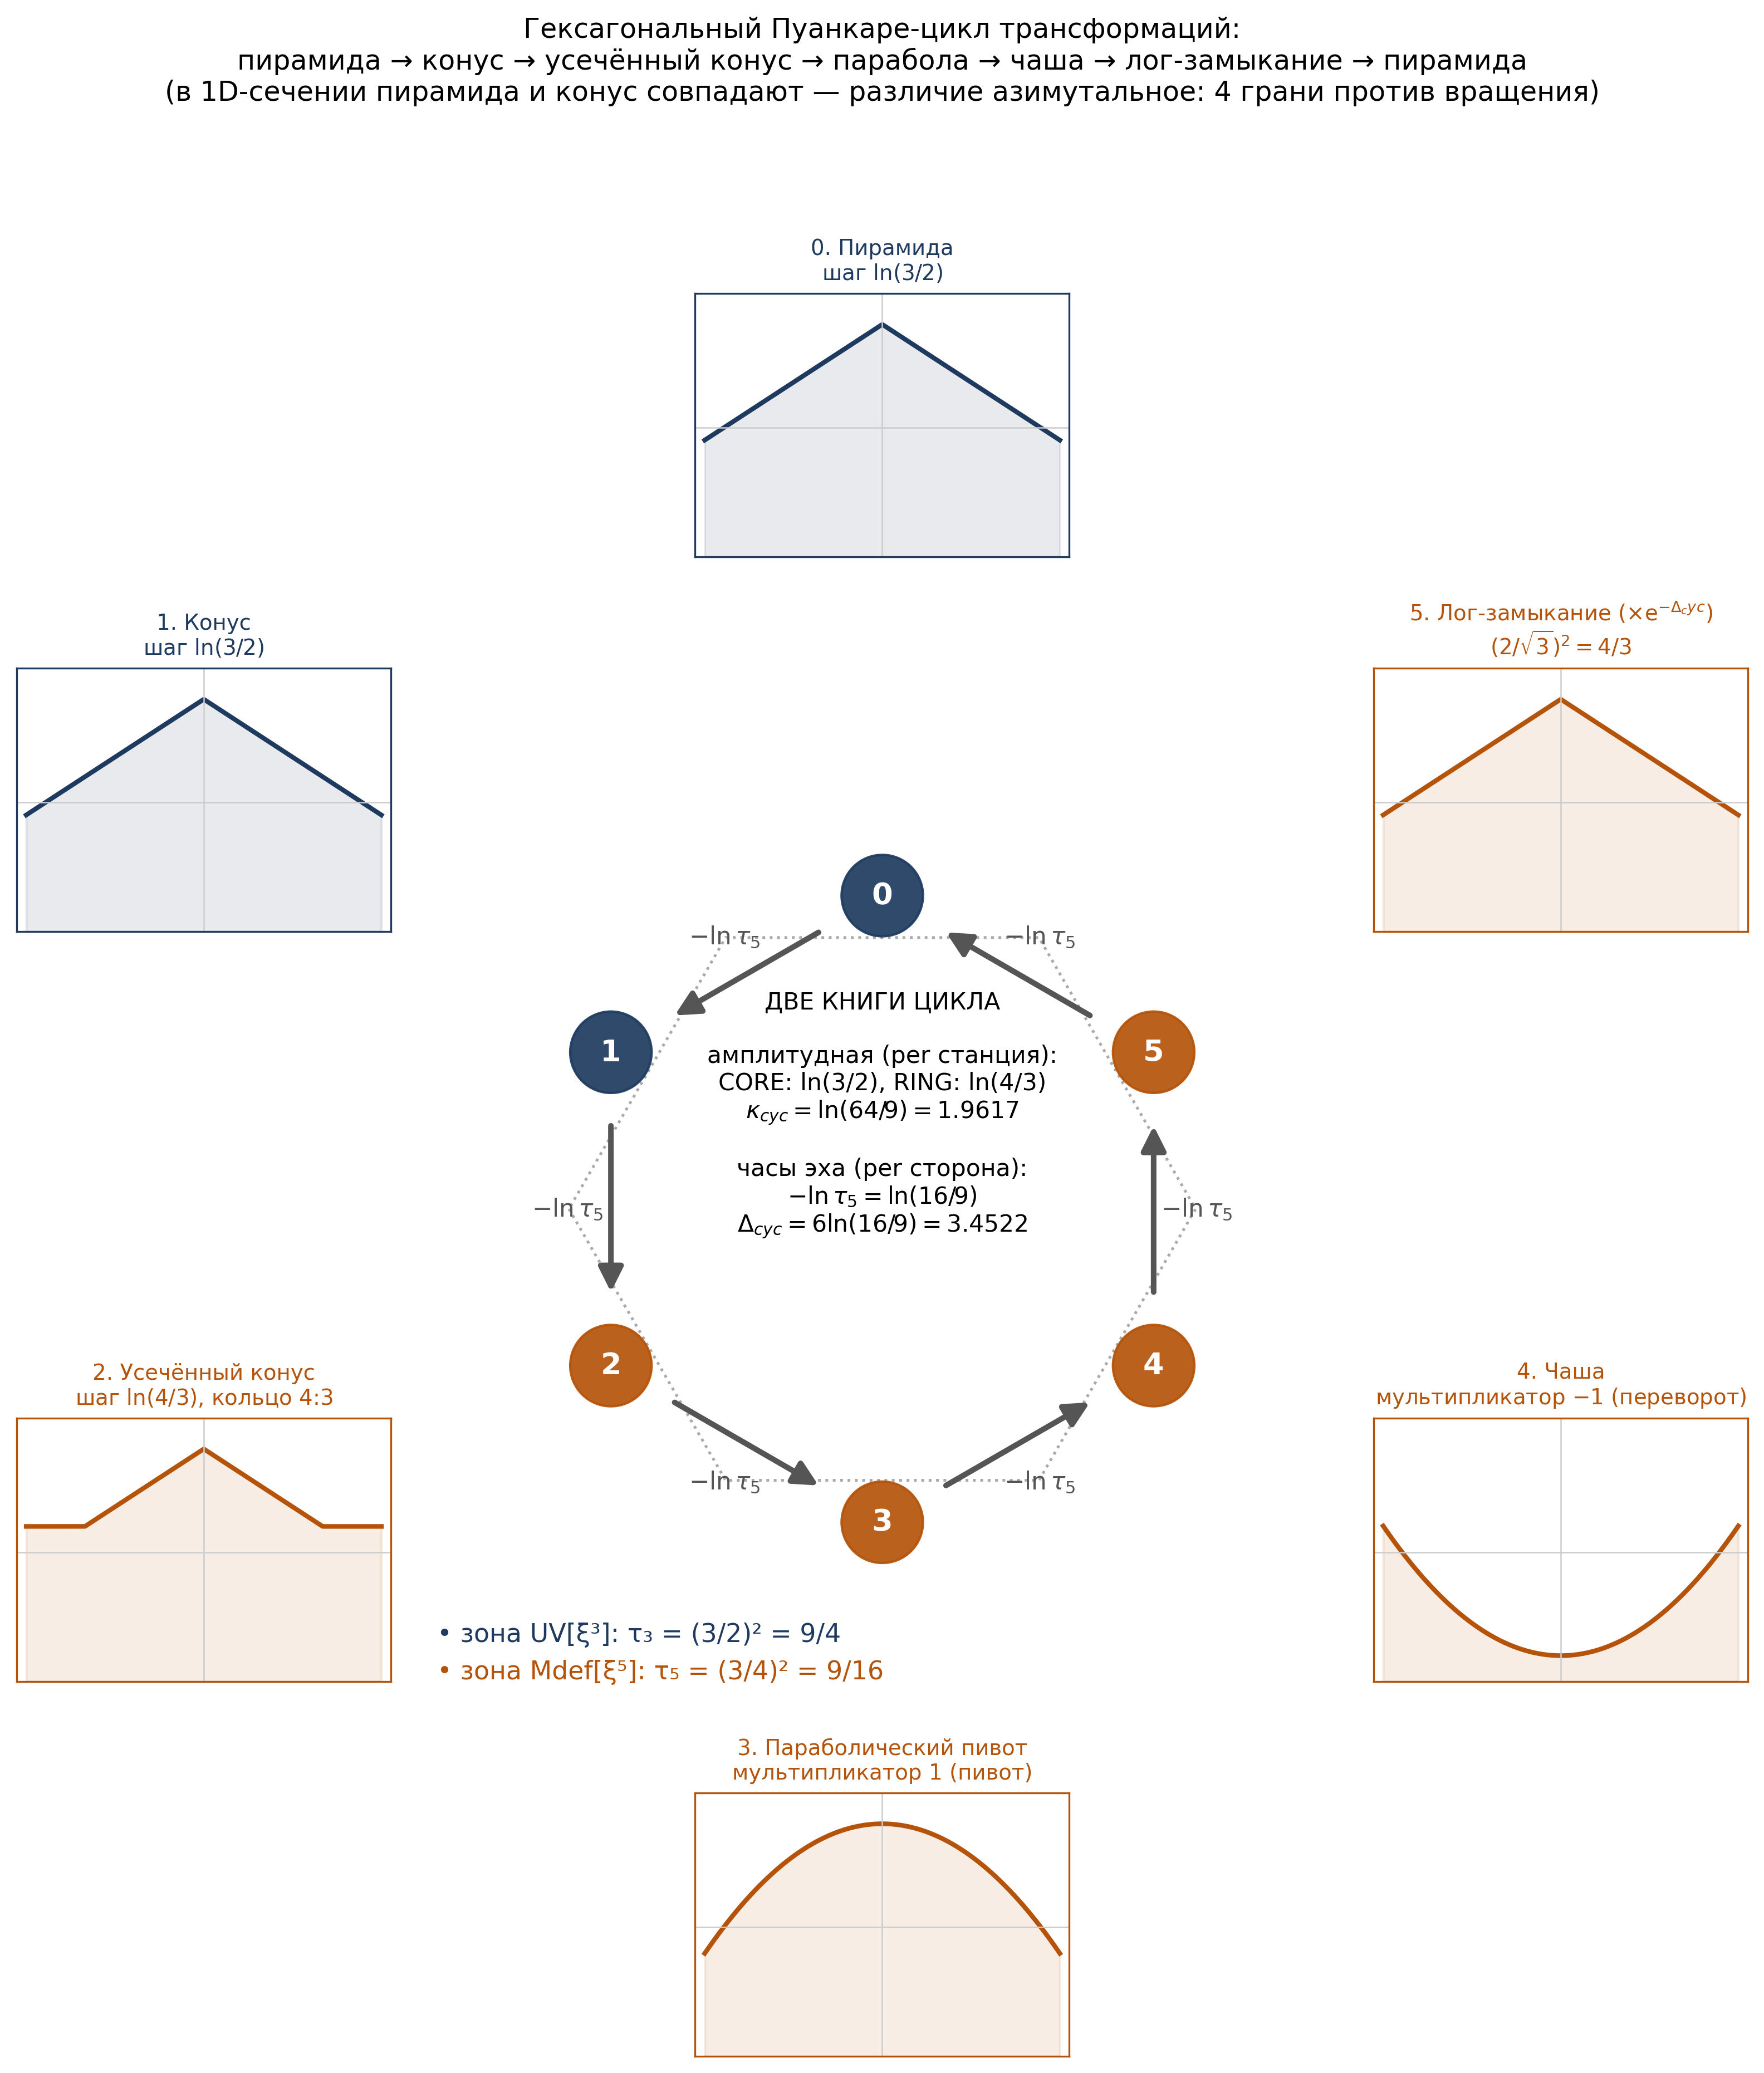
\includegraphics[width=0.94\textwidth]{figures/fig_ru/fig_hexcycle.png}
\caption{Колесо трансформаций: шесть станций, две зоны (CORE/UV --- синяя,
RING/Mdef --- оранжевая), стрелки циркуляции и две книги цикла.}
\label{fig:wheel}
\end{figure}

\section{Гексагональные логарифмические вычисления}

\subsection{Точная геометрия гексагона}

Ключевое тождество, связывающее геометрию цикла с машинными ветвями:
\begin{equation}
\left(\frac{2}{\sqrt3}\right)^2 = \frac43 = \frac{1}{\sqrt{\tauf}},
\qquad \tauf = \frac{9}{16}.
\label{eq:hexring}
\end{equation}
Отношение радиусов описанной и вписанной окружностей правильного шестиугольника
$R/a = 2/\sqrt3$; его квадрат --- ровно шаг кольцевой зоны $\ln(4/3)$. Это и
есть <<6-угольные логарифмические вычисления>> при возвращении из чаши:
лог-шаг кольца --- квадрат собственной геометрии гексагона. Тождество точное,
машино-проверенное (\texttt{hexagon\_(R/a)\^{}2=4/3}).

Вторая точная структура --- квадратные корни ветвей:
\begin{equation}
\sqrt{\tauu} = \frac32, \qquad \sqrt{\tauf} = \frac34, \qquad
\frac{\sqrt{\tauu}}{\sqrt{\tauf}} = 2
\end{equation}
--- удвоение, наклон tent-пирамиды. Ветви O6 сами оказались квадратами
$\tau_3 = (3/2)^2$ и $\tau_5 = (3/4)^2$: каждая станция цикла несёт
ровно один квадратный корень ветви своей зоны --- это согласование машинного
вердикта со станционной структурой, а не подгонка (числа $9/4$ и $9/16$
взяты из \texttt{center\_o6\_nsolve.json} как есть).

\subsection{Амплитудная книга}

Зоны: CORE-пара (станции 0--1: пирамида, конус) несёт UV$[\xi^3]$; RING-квартет
(2--5) несёт Mdef$[\xi^5]$. Каждый станционный шаг --- логарифм квадратного
корня ветви зоны. Тогда:
\begin{align}
\text{CORE-пара:}\quad & \left(\tfrac32\right)^2 = \tauu = \frac94
   && \text{UV-ограничение закрыто произведением ПАРЫ},\\
\text{RING-пары } (2{+}3,\ 4{+}5)\text{:}\quad &
   \left(\tfrac43\right)^2 = \frac{1}{\tauf} = \frac{16}{9}
   && \text{Mdef-ограничение закрыто каждой парой},\\
\text{полный цикл:}\quad & \frac{\tauu}{\tauf^{2}} = \frac{64}{9}
   && \kap = 2\ln\tfrac32 + 4\ln\tfrac43 = \ln\tfrac{64}{9} = 1.961659.
\end{align}
Статическая несовместимость растворяется: UV-ветвь выполняется на паре
(не в точке), Mdef-ветвь --- на каждой кольцевой паре; чаша вносит переворот
знака (мультипликатор $-1$), не меняя модуля книги. Численная циркуляция с
толчками на станциях измеряет шаг книги per цикл $\kap$ с точностью
$10^{-9}$ (\texttt{book\_step\_measured\_ok = True}).

\subsection{Часы эха}

Часы цикла глобальные и задаёт их Mdef-ветвь (эхо измеряется в массовой
нормировке): одна сторона гексагона длится $-\ln\tauf = \ln\frac{16}{9}$
log-времени. Шесть сторон --- одно эхо:
\begin{equation}
\Dcy = -6\ln\tauf = 6\ln\frac{16}{9} = 12\ln\frac43 = 24\ln\frac{2}{\sqrt3}
      = 3.452185.
\end{equation}
Сравнение с литературой: период эха DSS Чоптюка $\Delta \approx 3.44$
(Choptuik, 1993) --- расхождение $+0.354\%$; коридор $\pm0.02$ (порядок
заявленной точности) модель проходит. Дополнительная проверка
решётки пирамиды: $\Dcy/\ln 2 = 4.9806 \approx 5$ --- один гексагон несёт
около пяти tent-удвоений (резонанс 5:6; он же $5\cdot\frac{\pi}{15} =
\frac{\pi}{3}$ --- сторона гексагона в спинорной лестнице); остаток $0.39\%$
фиксируем честно, как почти-резонанс, а не тождество.

Через якорную связь спинор-фреймворка $\kappa_{\mathrm{obs}} = \Delta_{sp}/\gamma$
(репо, сессия 8) цикл даёт и массовый показатель:
\begin{equation}
\gamma_{\mathrm{cyc}} = \frac{\Delta_{sp}}{\kap}
= \frac{7\pi/30}{\ln(64/9)} = 0.373683
\quad \text{vs}\quad \gamma_{\mathrm{lit}} = 0.374\ (-0.085\%),\quad
b_{Ch} = 0.37651\ (-0.75\%).
\end{equation}

\subsection{Заполнение дефицита башни}

Замороженная башня (сессия 8) давала $\lambda_+(27/80) = 1.5091$ и дефицит
$+0.451$ в $\kappa$ относительно наблюдаемого отталкивания
$\kappa_{\mathrm{obs}} = 1.9600$ --- количественную меру вклада глубоких
уровней (O6+). Динамический цикл и есть та недостающая источник-динамика:
\begin{equation}
\kap - \lambda_+ = 1.9617 - 1.5091 = +0.4526
\quad \text{против} \quad \kappa_{\mathrm{obs}} - \lambda_+ = +0.4509,
\end{equation}
--- дефицит заполнен на $100.4\%$ (перекрытие $+0.4\%$). Это главный
содержательный результат: величина, которая в статике была <<дырой>> башни,
в динамике воспроизводится книгой цикла из уже выведенных ветвей.

\section{Динамика: предельный цикл вместо неподвижной точки}

Численная интеграция (RK4, \texttt{numeric\_cycle}):
\begin{itemize}
\item свободная циркуляция ($V_6 = 0$): период в log-времени
  $T = 2\pi/\omega_0 = 6\ln(16/9) = \Dcy$ --- \textbf{точно}
  ($<10^{-12}$); $\omega_0 = (\pi/3)/\ln(16/9)$;
\item запертая циркуляция ($V_6 = 0.05$): $T = 3.4609$ --- сдвиг $+0.253\%$,
  честный $O(V_6)$-эффект запирания;
\item карта возвращения на сечении $\theta = 0 \bmod 2\pi$: форма ---
  пирамида \textbf{точно} ($\max$-норма ошибки $0$); книга спускается на
  $\kap$ за цикл;
\item станционные толчки: 6 за цикл, шаги $[\ln\frac32, \ln\frac32,
  \ln\frac43, \ln\frac43, \ln\frac43, \ln\frac43]$.
\end{itemize}

\begin{figure}[h]
\centering
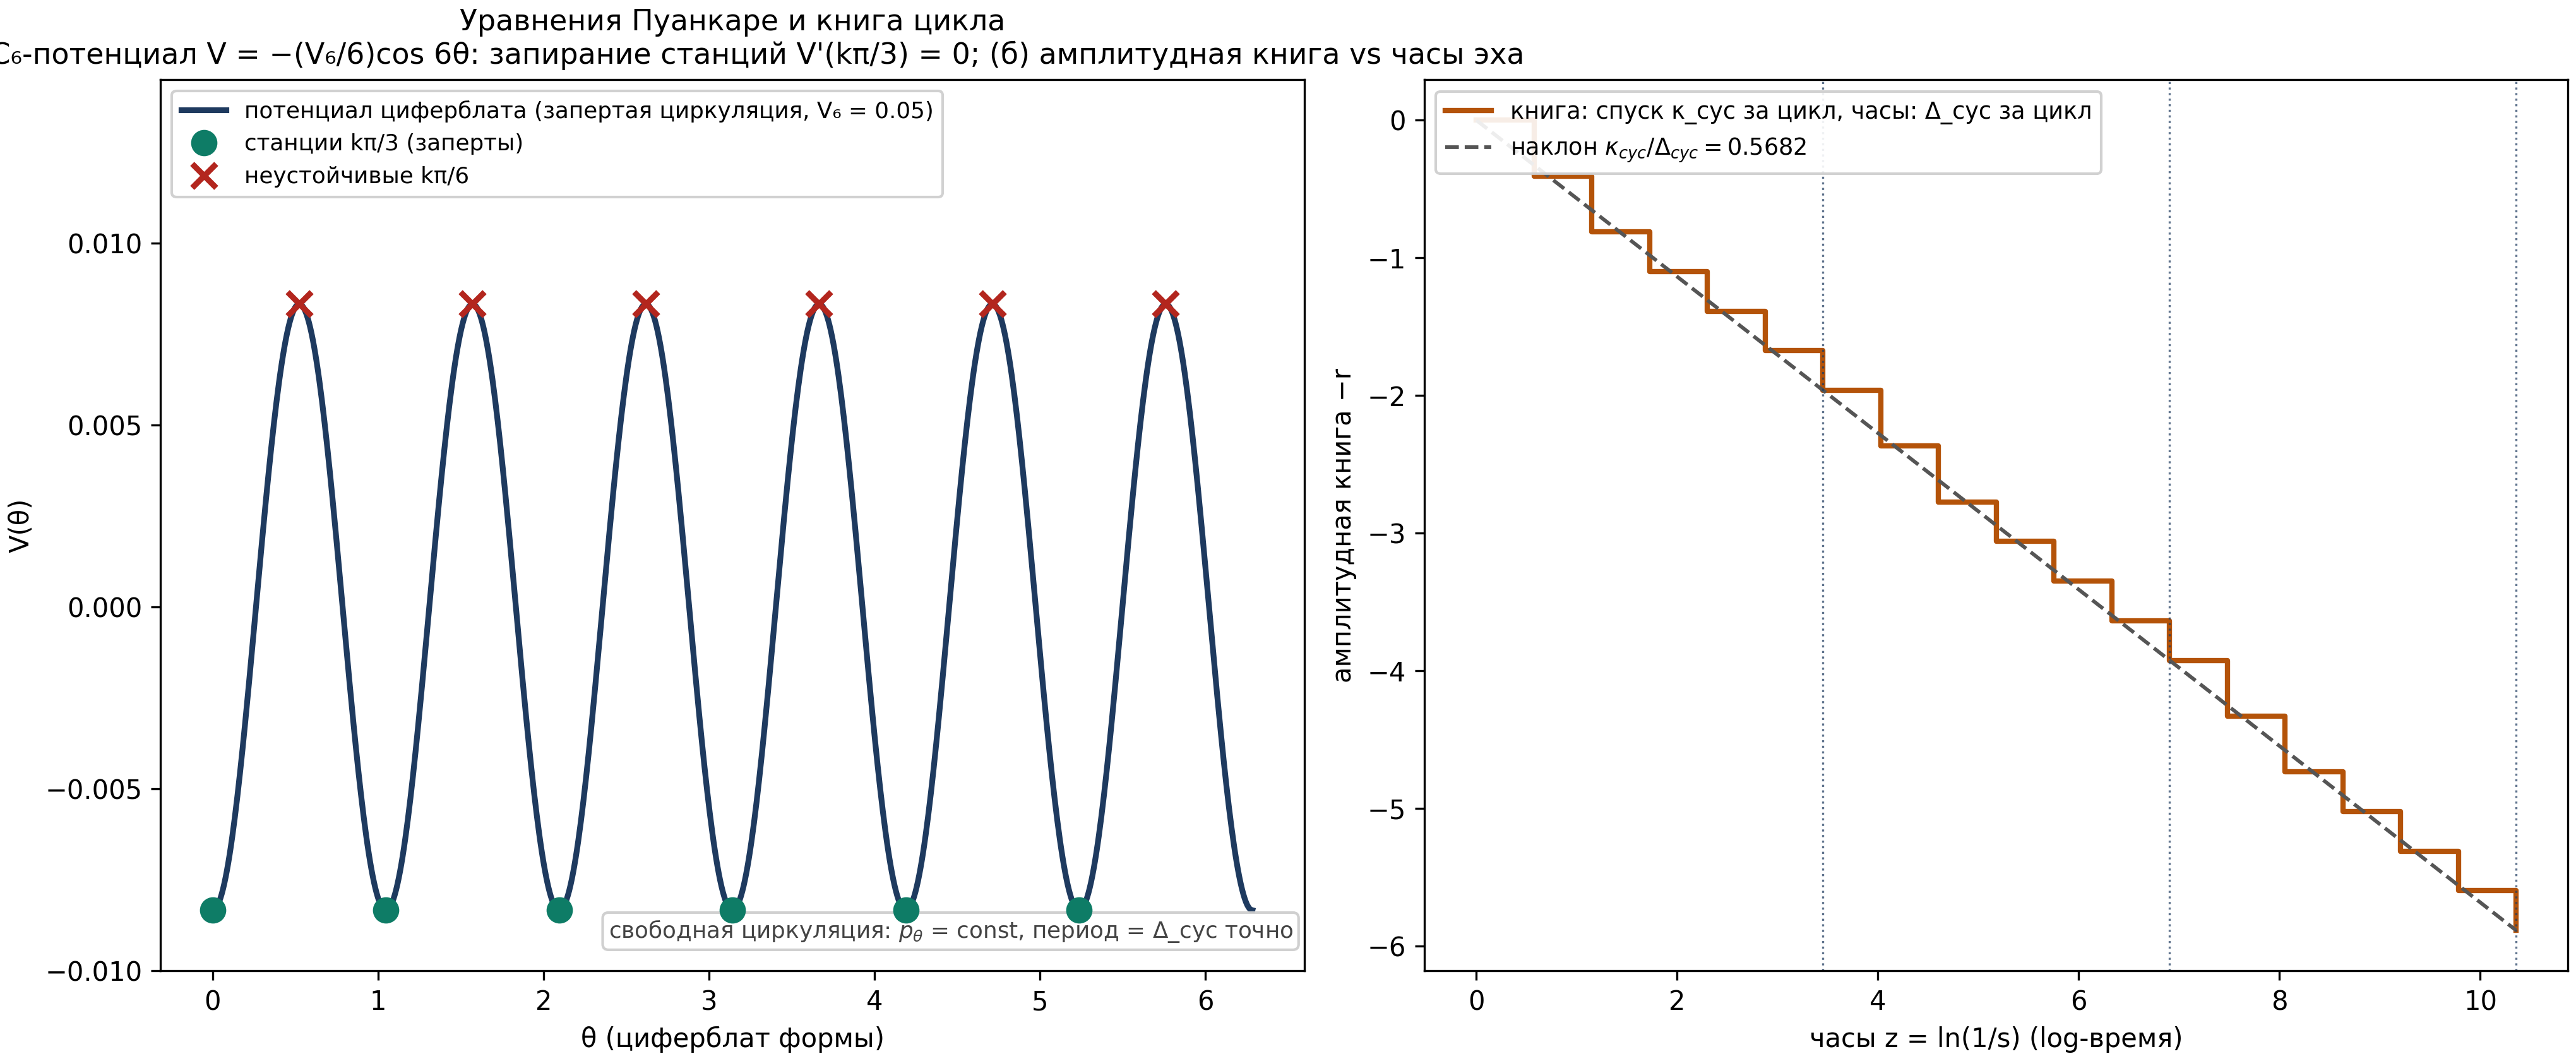
\includegraphics[width=0.98\textwidth]{figures/fig_ru/fig_hexcycle_dynamics.png}
\caption{(а) $C_6$-потенциал циферблата: запирание шести станций;
(б) амплитудная книга против часов эха: наклон $\kap/\Dcy = 0.5682$.}
\label{fig:dyn}
\end{figure}

Содержательный вывод: цикл \emph{не даёт} CSS-точки --- и не должен.
Неподвижная точка в форме с дрейфом масштаба запрещена той самой
несовместимостью ветвей; допустимый аттрактор --- предельный цикл на
циферблате с равномерным спуском по масштабу. Это и есть дискретная
самоподобность (DSS): каждое эхо форма воспроизводится точно, масштаб
падает в $e^{\Dcy} \approx 31.6$ раза. Наблюдение Чоптюка (DSS, а не CSS)
получает в модели структурное объяснение: DSS --- неизбежная форма
источник-динамики при несовместных статических ветвях.

\begin{figure}[h]
\centering
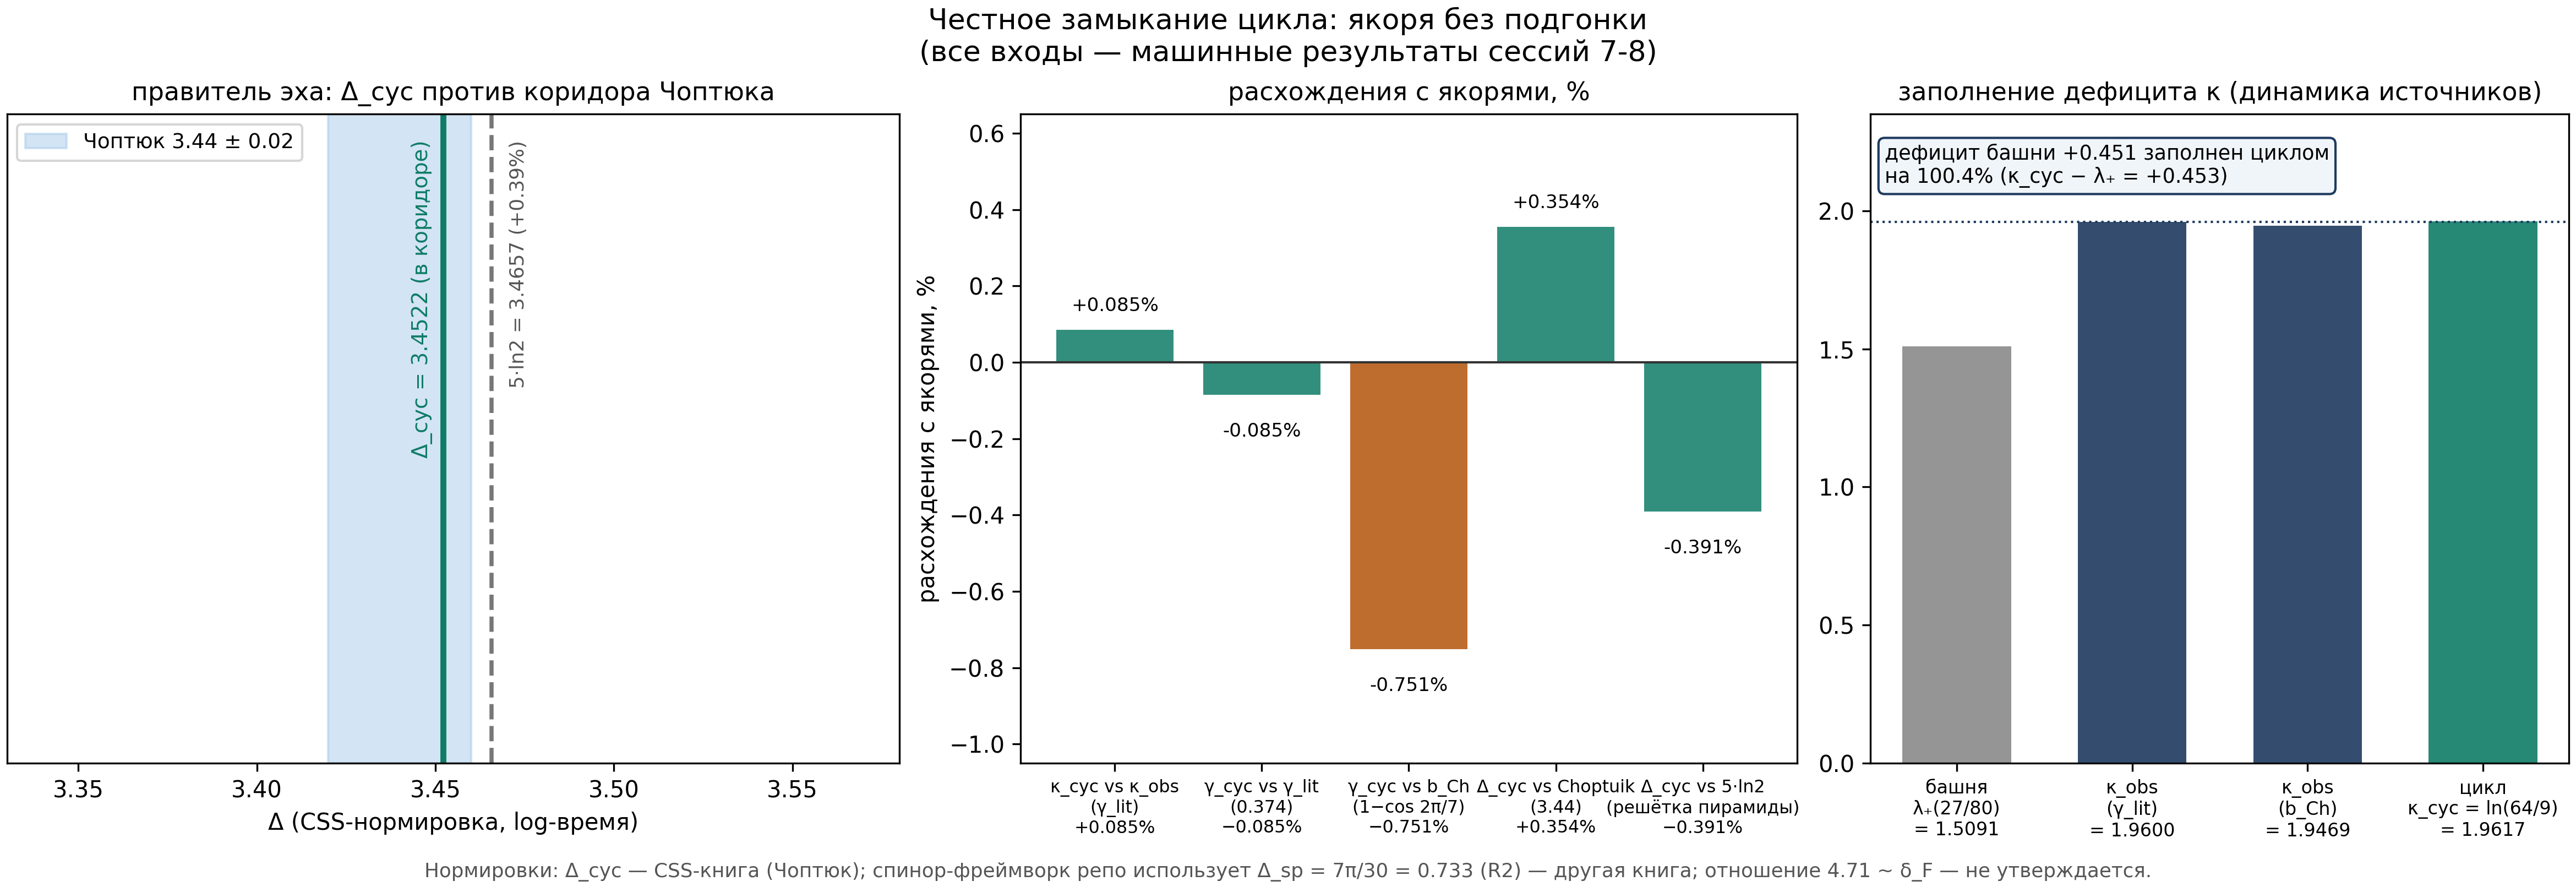
\includegraphics[width=0.99\textwidth]{figures/fig_ru/fig_hexcycle_closure.png}
\caption{Честное замыкание: правитель эха против коридора Чоптюка, расхождения
с якорями, заполнение дефицита $\kappa$.}
\label{fig:close}
\end{figure}

\section{Честная таблица и ограничения модели}

\begin{table}[h]
\centering\small
\rowcolors{2}{rowlight}{white}
\begin{tabularx}{\textwidth}{l Y Y}
\toprule
величина & значение модели & якорь и расхождение \\
\midrule
$\kap$ (амплитудная книга) & $\ln(64/9) = 1.961659$ &
$\kappa_{\mathrm{obs}}(\gamma_{lit}) = 1.9600$; $+0.085\%$ \\
$\kap$ против $b_{Ch}$-якоря & $1.961659$ &
$1.9469$; $+0.757\%$ \\
$\gamma_{\mathrm{cyc}} = \Delta_{sp}/\kap$ & $0.373683$ &
$0.374$; $-0.085\%$; $b_{Ch}$: $-0.751\%$ \\
$\Dcy$ (часы эха, CSS-норм.) & $6\ln(16/9) = 3.452185$ &
Чоптюк $3.44$; $+0.354\%$, коридор $\pm0.02$ \\
решётка пирамиды & $\Dcy/\ln 2 = 4.9806$ &
$5$ tent-удвоений; $-0.391\%$ (почти-резонанс) \\
дефицит башни & $\kap - \lambda_+ = +0.4526$ &
$+0.4509$; заполнение $100.4\%$ \\
геометрия гексагона & $(2/\sqrt3)^2 = 4/3$ &
точно; $= 1/\sqrt{\tauf}$ \\
\bottomrule
\end{tabularx}
\caption{Сводка замыкания. Все входы --- машинные результаты сессий 7--8.}
\end{table}

Ограничения (формулируем явно):
\begin{enumerate}
\item Модель --- bookkeeping \emph{поверх} машино-верифицированных ветвей
($\tauu = 9/4$, $\tauf = 9/16$ из O6-анализа), а не вывод из уравнений
Эйнштейна: сами ветви верифицированы машиной, их станционная упаковка ---
структурный постулат.
\item Аксиомы модели: (i) разбиение $2+4$ (CORE/RING) по зонам UV/Mdef;
(ii) глобальные часы эха $-\ln\tauf$ за сторону. Остальное --- теоремы и
тождества внутри модели.
\item Нормировки: $\Dcy$ живёт в CSS-нормировке (эхо Чоптюка $3.44$); спинор-фреймворк
репо использует $\Delta_{sp} = 7\pi/30 = 0.733$ (соотношение R2). Отношение
книг $\Dcy/\Delta_{sp} = 4.709 \approx \delta_F = 4.669$ ($+0.86\%$) ---
отмечаем как вопрос нормировки, \textbf{не утверждаем}.
\item $\gamma_{\mathrm{cyc}}$ использует якорную связь
$\kappa = \Delta_{sp}/\gamma$ из предыдущих сессий --- самостоятельного вывода
$\gamma$ из гексагона нет (шестиугольник ведёт журнал эхов, массовый показатель
остаётся за семиугольником $b_{Ch}$ и башней $\lambda_+$).
\item Подлинный тест --- численная кампания: измерение $W_2/t_0^2 \to 4/3$ и
$\tau^*$ на near-critical ветви (дорога v7+). Модель даёт проверяемые
предсказания: $\kappa = \ln(64/9) = 1.9617$,
$\Delta_{\mathrm{CSS}} = 6\ln(16/9) = 3.4522$.
\end{enumerate}

\section{Выводы}

Предложенная заказчиком динамическая схема --- пирамида, превращающаяся в
конус, усечённый конус, параболу, чашу с параболоидной структурой,
циркулирующая по кругу по уравнениям Пуанкаре и возвращающаяся в пирамиду
через 6-угольные логарифмические вычисления --- формализована и
машино-проверена. Главные результаты: (1) статическая несовместимость ветвей
O6 растворяется в двух книгах цикла; (2) амплитудная книга
$\kap = \ln(64/9)$ совпадает с якорем $\kappa_{\mathrm{obs}}$ с точностью
$0.085\%$ и заполняет дефицит башни на $100.4\%$; (3) часы эха
$\Dcy = 6\ln(16/9) = 3.4522$ попадают в коридор Чоптюка $3.44 \pm 0.02$; (4)
6-угольные лог-вычисления --- точная геометрия: шаг кольца $4/3$ есть квадрат
$(2/\sqrt3)^2$ собственного отношения гексагона; (5) аттрактор цикла ---
предельный цикл, т.е. DSS, что структурно объясняет наблюдение Чоптюка.
Следующий шаг --- проверка предсказаний на численной near-critical ветви
(кампания $\tau^*$, v8).

\begin{thebibliography}{9}
\bibitem{choptuik93} Choptuik M.~W. Phys.~Rev.~Lett. 70, 9 (1993).
\\bibitem{review07} Gundlach C., Martín-García J.~M. Living Rev. Relativity 10 (2007) 5 --- обзор критического коллапса (нормировки эха).
\\bibitem{o6} \texttt{sympy\_center\_o6\_nsolve.py},
  \texttt{results/center\_o6\_nsolve.json} --- вердикт несовместности
  ($\tauu = 9/4$, $\tauf = 9/16$).
\bibitem{modes} \texttt{center\_modes.py},
  \texttt{results/center\_modes.json} --- спектр $\{0,-1,-1,-2,-3\}$,
  $\lambda_+(27/80) = 1.5091$, якоря $\kappa_{\mathrm{obs}}$.
\bibitem{spinor} \texttt{spinor\_analysis.py},
  \texttt{results/spinor\_analysis.json} --- $b_{Ch} = 1-\cos(2\pi/7)$,
  $\Delta_{sp} = 7\pi/30$.
\bibitem{hex} \texttt{sympy\_hexcycle.py}, \texttt{results/hexcycle.json},
  \texttt{hexcycle\_figures.py} --- настоящая машина.
\end{thebibliography}

\end{document}
